

%%
%% This is file `ubcsample.tex',
%% generated with the docstrip utility.
%
% The original source files were:
%
% ubcthesis.dtx  (with options: `ubcsampletex')
%% 
%% This file was generated from the ubcthesis package.
%% --------------------------------------------------------------
%% 
%% Copyright (C) 2001
%% Michael McNeil Forbes
%% mforbes@alum.mit.edu
%% 
%% This file may be distributed and/or modified under the
%% conditions of the LaTeX Project Public License, either version 1.2
%% of this license or (at your option) any later version.
%% The latest version of this license is in
%%    http://www.latex-project.org/lppl.txt
%% and version 1.2 or later is part of all distributions of LaTeX
%% version 1999/12/01 or later.
%% 
%% This program is distributed in the hope that it will be useful,
%% but WITHOUT ANY WARRANTY; without even the implied warranty of
%% MERCHANTABILITY or FITNESS FOR A PARTICULAR PURPOSE.  See the
%% LaTeX Project Public License for more details.
%% 
%% This program consists of the files ubcthesis.dtx, ubcthesis.ins, and
%% the sample figures fig.eps and fig.fig.
%% 
%% This file may be modified and used as a base for your thesis without
%% including the licence agreement as long as the content (i.e. textual
%% body) of the file is completely rewritten. You must, however, change
%% the name of the file.
%% 
%% This file may only be distributed together with a copy of this
%% program. You may, however, distribute this program without generated
%% files such as this one.
%% 
% This Sample thesis requires \LaTeX2e
\NeedsTeXFormat{LaTeX2e}[1995/12/01] \ProvidesFile{ubcsample.tex}[2010/12/09 v1.68 ^^J University of British Columbia Sample Thesis]

% This is the \documentclass[]{} command.  The manditory argument
% specifies the "flavour" of thesis (ubcthesis for UBC).  The
% optional arguments (in []) specify options that affect how the
% thesis is displayed.  Please see the ubcthesis documentation for
% details about the options.
\documentclass[msc,oneside]{ubcthesis}

%
% To compile this sample thesis, issue the following commands:
% latex ubcsample
% bibtex ubcsample
% latex ubcsample
% latex ubcsample
% latex ubcsample
%
% To view use xdvi (on unix systems):
% xdvi ubcsample.dvi
%
% To make a postscript file, use dvips:
% dvips -o ubcsample.ps ubcsample.dvi
%
% To view the postscript file, use ghostview or gv (on unix systems):
% gv ubcsample.ps
%
%************************************************
% Optional packages.
%
% The use of these packages is optional, but they provide various
% tools for more flexible formating.  The sample thesis uses these,
% but if you remove the example code, you should be able to exclude
% these packages.  Only standard packages have been described here;
% they should be installed with any complete LaTeX instalation, but
% if not, you can find them at the Comprehensive TeX Archive Network
% (CTAN): http://www.ctan.org/
%
%******** afterpage ***************************
% This package allows you to issue commands at the end of the current
% page.  A good use for this is to use the command
% \afterpage{\clearpage} right after a figure.  This will cause the
% figure to be inserted on the page following the current one (or on
% the current page if it will fit) but will not break the page in the
% middle.
\usepackage{afterpage}

%******** float *********************************
% This package allows you to customize the style of
% "floats"---floating objects such as figures and tables.  In
% addition, it allows you to define additional floating objects which
% may be included in a list similar to that produces by \listoftables
% and \listoffigures.  Common uses include introducing floats for
% programs and other code bits in Compute Science and Chemical Schema.
\usepackage{float}

%******** tocloft *******************************
% This package allows you to customize and define custom lists such
% as a list of programs or Chemical Scheme.  Note: if you use the
% subfigure package, you must specify that you do as an option here.
% The title option uses the default formatting.  We do not use this
% here as the default formatting is acceptable.  Use the float
% package instead unless you need the extra formatting control
% provided by tocloft.
%\usepackage[subfigure, titles]{tocloft}
%******** alltt *********************************
% The alltt package allows you to include files and have them
% formatted in a verbatim fashion.  This is useful for including
% source code from an additional file.
%\usepackage{alltt}
%******** listings ******************************
% The listings package may be used to include chunks of source code
% and has facilities for pretty-printing many languages.
%\usepackage{listings}
%******** longtable *****************************
% The longtable package allows you to define tables that span
% multiple pages.
\usepackage{longtable}

%******** graphics and graphicx *****************
% This allows you to include encapsulated postscript files.  If you
% don't have this, comment the \includegraphics{} line following the
% comment "%includegraphics" later in this file.
\usepackage{graphicx}
\graphicspath{{./images/}}

%******** subfigure *****************************
% The subfigure package allows you to include multiple figures and
% captions within a single figure environment.
%\usepackage{subfigure}
%******** here **********************************
% The here package gives you more control over the placement of
% figures and tables.  In particular, you can specify the placement
% "H" which means "Put the figure here" rather than [h] which means
% "I would suggest that you put the figure here if you think it looks
% good."
%\usepackage{here}
%******** pdflscape ********************************
% This allows you to include landscape layout pages by using the
% |landscape| environment.  The use of |pdflscape| is preferred over
% the standard |lscape| package because it automatically rotates the
% page in the pdf file for easier reading.  (Thanks to Joseph Shea
% for pointing this out.)
\usepackage{pdflscape}

%******** natbib ********************************
% This is a very nice package for bibliographies.  It includes options
% for sorting and compressing bibliographic entries.
\usepackage[numbers,sort&compress]{natbib}

%******** psfrag ******************************
% This allows you to replace text in postscript pictures with formated
% latex text.  This allows you to use math in graph labels
% etc. Uncomment the psfrag lines following the "%psfrag" comment
% later in this file if you don't have this package.  The replacements
% will only be visible in the final postscript file: they will be
% listed in the .dvi file but not performed.
\usepackage{psfrag}

%******** hyperref *****************************
% Please read the manual:
% http://www.tug.org/applications/hyperref/manual.html
%
% This adds hyperlinks to your document: with the right viewers (later
% versions of xdvi, acrobat with pdftex, latex2html etc.) this will
% make your equation, figure, citation references etc. hyperlinks so
% that you can click on them.  Also, your table of contents will be
% able to take you to the appropriate sections.  In the viewers that
% support this, the links often appear with an underscore.  This
% underscore will not appear in printed versions.
%
% Note: if you do not use the hypertex option, then the dvips driver
% may be loaded by default.  This will cause the entries in the list
% of figures and list of tables to be on a single line because dvips
% does not deal with hyperlinks on broken lines properly.
%
% NOTE: HYPERREF is sensitive to the ORDER in which it is LOADED.
% For example, it must be loaded AFTER natbib but BEFORE newly
% defined float environments.  See the README file with the hyperref
% for some help with this.  If you have some very obscure errors, try
% first disabling hyperref.  If that fixes the problem, try various
% orderings.
%
% Note also that there is a bug with versions before 2003/11/30
% v6.74m that cause the float package to not function correctly.
% Please ensure you have a current version of this package.  A
% warning will be issued if you leave the date below but do not have
% a current version installed.
%
% Some notes on options: depending on how you build your files, you
% may need to choose the appropriate option (such as [pdftex]) for the
% backend driver (see the hyperref manual for a complete list).  Also,
% the default here is to make links from the page numbers in the table
% of contents and lists of figures etc.  There are other options:
% excluding the [linktocpage] option will make the entire text a
% hyperref, but for some backends will prevent the text from wrapping
% which can look terrible.  There is a [breaklinks=true] option that
% will be set if the backend supports (dvipdfm for example supports
% it but does not work with psfrag.)
%
% Finally, there are many options for choosing the colours of the
% links.  These will be included by default in future versions but
% you should probably consider changing some now for the electronic
% version of your thesis.
\usepackage[unicode=true, linktocpage, linkbordercolor={0.5 0.5 1}, citebordercolor={0.5 1 0.5}, linkcolor=blue]{hyperref}

% If you would like to compile this sample thesis without the
% hyperref package, then you will need to comment out the previous
% \usepackage command and uncomment the following command which will
% put the URL's in a typewriter font but not link them.
%\newcommand\url[1]{\texttt{#1}}
%******** setspace *******************************
% The setspace package allows you to manually set the spacing of the
% file.  UBC may require 1.5 spacing for microfilming of theses.  In
% this case you may obtain this by including this package and issuing
% one of the following commands:
%\usepackage{setspace}
%\singlespacing
%\onehalfspacing
%\doublespacing
% These commands are optional.  The defaults are shown.  You only
% need to include them if you need a different value
\institution{The University Of British Columbia}

% If you are at the Okanagan campus, then you should specify these
% instead.
%\faculty{The College of Graduate Studies}
%\institutionaddress{Okanagan}
\faculty{The Faculty of Electrical and Computer Engineering} \institutionaddress{Vancouver}

% You can issue as many of these as you have...
\previousdegree{B.ScEng, The University of New Brunswick, 2008}

% You can override the option setting here.
\degreetitle{Masters of Applied Science}

% These commands are required.
\title{mHot} \subtitle{Mobile Here or There - A framework for runtime offloading of computation from mobile devices to the cloud.} 
\author{William Joseph Gaudet} \copyrightyear{2011} \submitdate{\monthname\ \number\year} 

% The "\ " is required after
% \monthname to prevent the
% command from eating the space.
\program{Engineering}

% These commands are presently not required for UBC theses as the
% advisor's name and title are not presently required anywhere.
%\advisor{Ariel R.~Zhitnitsky}
%\advisortitle{Professor of Physics}
% One might want to override the format of the section and chapter
% numbers.  This shows you how to do it.  Note that the current
% format is acceptable for submission to the FoGS: If you wish to modify
% these, you should check with the FoGS explicity. prior to making
% the modifications.
\renewcommand\thepart {\Roman{part}} 
\renewcommand\thechapter {\arabic{chapter}} 
\renewcommand\thesection {\thechapter.\arabic{section}} 
\renewcommand\thesubsection {\thesection.\arabic{subsection}} 
\renewcommand\thesubsubsection{\thesubsection.\arabic{subsubsection}} 
\renewcommand\theparagraph {\thesubsubsection.\arabic{paragraph}} 
\renewcommand\thesubparagraph {\theparagraph.\arabic{subparagraph}}

\setcounter{tocdepth}{2} \setcounter{secnumdepth}{2}

% Here is an example of a "Program" environment defined with the
% "float" package.  The list of programs will be stored in the file
% ubcsample.lop and the numbering will start with the chapter
% number.  The style will be "ruled".
\floatstyle{ruled} 
\newfloat{Program}{htbp}{lop}[chapter]

% Here is the start of the document.
\begin{document}

%% This starts numbering in Roman numerals as required for the thesis
%% style and is mandatory.
\frontmatter

%%% The order of the following components should be preserved.  The order
%%% listed here is the order currently required by FoGS:        \\
%%% Title (Mandatory)                                           \\
%%% Preface (Manditory if any collaborator contributions)       \\
%%% Abstract (Mandatory)                                        \\
%%% List of Contents, Tables, Figures, etc. (As appropriate)    \\
%%% Acknowledgements (Optional)                                 \\
%%% Dedication (Optional)                                       \\
\maketitle 

%% Mandatory
\begin{abstract}
	
	%% Mandatory -  maximum 350 words
	Today the average north american carries a computer several orders of magnitude more powerful than the computer used to guide the Apollo space craft to the moon and safely back. However, with this dramatic increase in both ubiquity and power of personal mobile computing, has come a host of applications that require significantly more computational power than is available in today's smart phones. Additionally, battery life of mobile devices is still a significantly limiting factor when doing large quantities of computation on mobile platforms.
	
	With these factors in mind this research investigates the gains in performance, quality of computation, and battery life which can be made possible by real time offloading of computation from a mobile device to a server platform.
	
	Furthermore, it details the design and implementation of a framework for offloading computation from mobile devices which has at its core the goal of limiting the cognitive overhead for the developer to conduct such an offload.
\end{abstract}

\tableofcontents 

%% Mandatory
\listoftables 

%% Mandatory if thesis has tables
\listoffigures 

%% Mandatory if thesis has figures
\listof{Program}{List of Programs} 

%% Optional
%% Any other lists should come here, i.e.
%% Abbreviation schemes, definitions, lists of formulae, list of
%% schemes, glossary, list of symbols etc.
\chapter{Acknowledgements} 

%% Optional
\chapter{Dedication} 

%% Optional
% Any other unusual prefactory material should come here before the
% main body.
% Now regular page numbering begins.
\mainmatter

% Parts are the largest structural units, but are optional.
%\part{Thesis}
\chapter{Introduction} 

% (fold)
\label{chap:introduction}
\subsection*{Motivations} % (fold)
\label{sub:motivations}

Desktop and laptop computers have been the mainstay of personal computing for more than 30 years, providing untold utility to millions of users worldwide. However, due to recent improvements in battery technology paired with reduction in size and cost of the components necessary to build a computer system, industry leaders are declaring the "Death of the PC" and subsequent rise of mobile platforms, referring to smartphones and tablet computers rather than laptops. At the All Things Digital Conference 2010 Steve Jobs, founder and CEO of Apple, echoed this sentiment, stating that Personal Computers (PCs) would become like trucks: they will still exist but the bulk of people won't need them.

Additionally, this new era of pervasive mobile computing has given rise to a suite of new mobile applications, with the average smartphone boasting the equivalent computational capability of a PC from 2001, the potential for innovative new applications seems limitless---this is aided by the many environmental sensors present on the typical smart phone such as those which measure position, orientation, and acceleration.

There is however a second class of application that requires significantly greater capabilities than are offered by the current generation of mobile platforms. An example of this class of application include music recognition programs such as Shazam [CITATION] which requires a large corpus of music against which to compare an audio sample, additionally the digital signal processing requirements are likely greater than the capabilities of the mobile device (or they process would be prohibitively non performant on the mobile device). In spite of these limitations, these applications exist and provide a great deal of utility to the end user. The shortcomings of the mobile devices are addressed through the offloading of the more challenging computational work to a computer with greater resources and capabilities at its disposal---This process will henceforth be referred to computational offloading. The benefits of computational offloading are seemingly obvious; providing the user the facade of having a more performant computer than they already have. In fact computation offload is not a new idea, search systems such as Google can be viewed as computational offloading systems. Whereby the user provides a search string into the google web portal, which has significantly more capabilities and data at its disposal, and google returns a listing of search results.

Currently if a developer wants to add some computational offloading to their mobile application, they must explicitly construct their own method for offloading their data structures, additionally they must engineer a remote runtime to accept the offloaded data, execute the remote operations, and return the results to the mobile device. This gives rise to a large number of potential problems for a developer. There are many parameters which must be considered when offloading computation, not the least of which is the bandwidth of the remote connection. In a mobile scenario there is a delicate balance between the bit rate of the connection and the power consumption costs (watts/byte) which must be considered when determining the value of a computation offload. Often times these complexities give rise to incomplete or inefficient solutions, as the developer may lack the experience and skill to create a reasonable offloading system.

The goal of this work is two fold, to identify the critical parameters which must be taken into account in order to develop a decision model for offloading computation, and to describe and implement a framework for the android mobile platform which limits the cognitive overhead for the developer when creating mobile applications which require computation offloading. 
% subsection motivations (end)

\subsection{Decision Goals} % (fold)
\label{sub:decision_goals}
The decision model described in this work will focus around three goals, minimizing runtime, maximizing computation 'quality', and maximizing battery life. Minimizing runtime is a fairly straightforward goal, the decision to offload computation can be made trivially by predicting the which platform will have the lowest runtime (the following equation is used).

\begin{equation}
	min(T_{compRemote} + T_{transmission}, T_{compLocal})
\end{equation}
 
Computation quality is considered in a special case of problem, where an increased number of iterations of a particular problem would increase the correctness of a solution. An example of this would be an iterative root finding method, where more iterations would lead to a more correct result (a value closer to the actual root). In the case of a mobile computation offloading situation, one could reason that if a problem were executed in the same approximate running time but on server with increased capabilities the over all quality of the computation could be increased. Or put a different way, given a boundary of some level of quality of result, the running time could be minimized.

\begin{equation}
	min(T_{compRemoteToQuality(q)} + T_{transmission}, T_{compLocalToQuality(q)})
\end{equation}

Finally in general the goal of reducing battery life can be expressed simply as:

\begin{equation}
	min(P_{compLocal}, P_{transmission})
\end{equation}

where P is the cost in watts of a particular operation.

% subsection decision_goals (end)

\subsection*{Development Overhead} % (fold)
\label{sub:development_overhead}

Minimizing the cognitive overhead of developers is the goal of most development frameworks, reducing the amount of work a developer has to do both in lines of code and in adjusting their mental picture of a problem in order to solve it is in general viewed as desirable. The design of this framework has limited the amount of input from the developer to a sole annotation on a method, the use of some custom data structures when building their domain objects, and the following of some development best practices. These will all be described at length in the design and implementation section of this document.

% subsection development_overhead (end)

% chapter introduction (end)

\chapter{Background and Previous Work} % (fold)
As was stated in the introduction, computational offload is not a novel concept per say. There are several applications available to smart phone users today that make use of computational offloading to provide a more rich experience to the end user. Shazam was one such application, where a user records a section of music and the app sends the recording to a server for identification. [ADD SOME MORE EXAMPLES]

Cuervo et al \cite{Cuervo:2010}, presented their framework MAUI, which allowed for runtime offloading of mobile computation from the windows platform. The MAUI framework sought to maximize battery life by determining at runtime which problems could be executed remotely on a parallel runtime. However their approach had some flaws, their decision to allow the developer to use regular primitive data types and rely on reflection and serialization to ship their objects to the remote server while desirable for the developer in terms of ease of use, the use of reflection and serialization incur processor overheads which contribute to the power cost of the object transmission.

% chapter background (end)
\label{chap:background}


% chapter literature_review (end)
\chapter{Design and Modelling} 

% (fold)
\label{chap:design_modelling}

\section{Overview} 

% (fold)
\label{sec:overview}

% section overview (end)
\section{A Framework for Data Migration} 
\label{sec:a_framework_for_data_migration}

\subsection{Dynamic Proxies} % (fold)
\label{sub:dynamic_proxies}

The primary mechanism for abstracting the decision of where to execute a method (in the cloud or on the mobile device) is the Java Dynamic Proxy class [citation]. The dynamic proxy class enables runtime proxing of any object provided it implements an interface. A dynamic proxy object then implements the interface of the object to be proxied at runtime, and then routes all method calls through its invoke method. It is in this invoke method that the decision to either package the object graph and ship it to the server for execution or execute locally is made. 

The dynamic proxy class does have some shortcomings, it requires developers to create interfaces for the methods they want to to be remotable, additionally the developer must explicitly create the proxy objects for use in their code, and finally dynamic proxies do incur a performance overhead. Simple running time experiments show that the average time cost of a regular Java method invocation is approximately 60ns while the average time cost of the same method invocation done through a dynamic proxy object is around 5ms. However with these costs in mind a developer can make architectural decisions to help mitigate these performance overheads. The shortcomings with respect to the use of interfaces is actually viewed as a positive as it forces the developer towards best practices of programming to interfaces and not implementation. Finally steps have been taken to mitigate developer pain with regards to creation and use of dynamic proxies, by way of the Java Generics system every object which descends from the AbstractRemoteObject has a factory method which will wrap the object in a proxy.

% subsection dynamic_proxies (end)

% (fold)

\subsection*{Remote Method Invocation} 
\label{sub:remote_method_invocation}

When mHot determines that a method should be executed in the cloud rather than locally on the mobile device, it must conduct a remote method invocation. While it takes its name from the Java RMI system, the remote method invocation object is only related to RMI in the fact that it allows for a developer to remotely invoke methods on an object. The Java RMI system is a fully feature interprocess communication system and as such when mHot was first designed RMI was investigated as a potential solution to the problem of object transmission and method invocation. However, the lack of support for native RMI in the Android platform was seen as an insurmountable barrier. As such, a custom and lightweight remote invocation methodology was devised with a goal in mind to minimize both the amount of computation required to marshal the objects between the compute platforms and limit the amount of data that would be transmitted over the wire---this is particularly important due to battery life constraints and the substantial energy costs of the high bandwidth radios (3g / WiFi).

A single remote invocation is a collaboration between three objects, the target remotable object, the argument array, and the result. Each object plays a particular role in the method invocation process, and together make up the composition of a RemoteInvocationMethod object. The target remotable object is the object against which the method will be invoked, the argument array contains facilities for serializing and deserializing the arguments the method takes---these objects must be either primitive data types, or implement RemoteableObject otherwise an exception will be thrown---, finally the result is container for the returned result of the method. The remote method invocation process is performed by the Remote Dynamic Proxy Object, this process is outlined in the activity diagram shown in Figure \ref{fig:RMI-Activity-Diagram}. Presently the remoted method should not mutate the target object's state as mHot has no facilities for returning the object once it's been shipped to the remote server, thus the developer must currently take that into account when designing their APIs. However this could reasonably be addressed via some post execution synchronization mechanism, or by returning the mutated object as the result---though this would be a poor stop gap solution as it would increase the amount of traffic on the line.

\begin{figure}
	\centering
	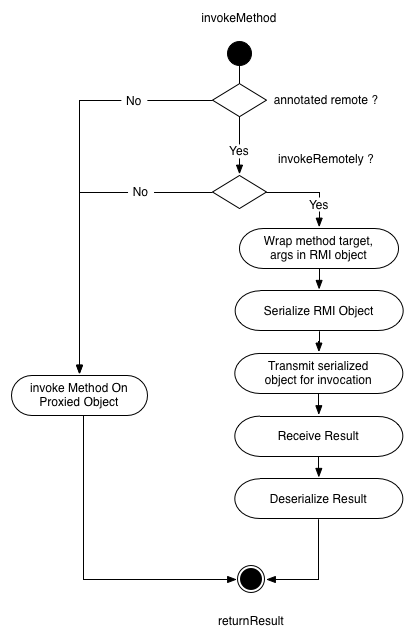
\includegraphics[width=0.75\textwidth]{RMI-Activity-Diagram}
	\caption{An Activity Diagram showing the RMI invocation process}
	\label{fig:RMI-Activity-Diagram}
\end{figure}

% (fold)

% subsection remote_method_invocation (end)
\subsection*{Data Serialization} 

% (fold)
\label{sub:data_serialization}

When a dynamic proxy object receives a method invocation that has been tagged as remotable, if the framework has determined that the request should be executed remotely, the proxied object must first be serialized before it can be shipped to the server. The proxied object can take on one of two forms: a simple object composed only of primitive data types (integers, floating point numbers, booleans etc) or a complex object graph composed of zero or more primitive types and one or more references to other objects. These other objects may in turn also contain references to additional objects both complex and simple as well as cyclical references between objects. 

Given the cost associated with object serialization both in terms of computation (due to memory allocation and object graph graph traversal) and in terms of communications bandwidth the task of the object serializer becomes two fold. Most importantly it must correctly serialize the object graph preserving any and all object references (including circular ones); additionally the serializer must attempt to minimize the size of the transmitted object graph.

This is primarily done by the encapsulation of an object's fields in container object which implements the RemotableField<T> interface. [CODE LISTING] The interface exposes several values about the encapsulated object all of which are required to correctly and efficiently (in both space and time) serialize the object graph, the more relevant methods to the serialization process are the following:
\begin{itemize}
	\item int size() - Returns the size in bytes required to serialize this field (in the implemented case of a RemoteFieldObject this is 4 bytes for the reference to the object) 
	\item <T> get() - Returns the object which is encapsulated in this field, in the case of a primitive value it is wrapped in it's Java object container type (Integer for int) etc, due to performance issue with the autoboxing system [CITATION NEEDED] where T is either a primitive data type or an implementation of RemoteObject 
	\item boolean isDirty() - Returns true if this object has had it's value set since initialization or last serialization - this is used to minimize the amount of data that must be transmitted to the remote server. 
	\item void Serialize(ByteBuffer) - Serializes the field to the provided ByteBuffer 
	\item void Deserialize(ByteBuffer) - Deserializes the field from the provided ByteBuffer 
	\item FieldVisitor acceptVisitor(FieldVisitor) - Accepts the field visitors which are used to conduct a variety of tasks in the graph serialization process. 
\end{itemize}

\subsection*{The Serialization Process} 

% (fold)
\label{sub:the_serialization_process}

The object serialization process is a modified depth first search. In effect the process visits every node in the graph twice, once to compute the overall size required to encode the graph as a binary representation, and a second time to perform the serialization it self. [This is a potential future work situation, some of this could probably be improved]. 

When a object in the graph is visited by the size computation pass, each of the object's remotable fields are interrogated for their serialization size---It should be noted that the fields for each object class are stored in a memoization cache to prevent recalculation of the classes' remotable fields through the use of the Java reflection APIs which are not very performant [Maybe this should be a footnote probably needs a citation]. If the field encapsulates a primitive field it simply looks up the serialization size cost for that field which is its data size in addition to the field reference, however, if the field encapsulates a remotable object it either adds 8 bytes if it has been visited once before---the byte cost of referencing an object which has already been visited---or it adds 8 bytes plus the serialization cost of that object, which is computed immediately---A complete list of default data type serialization costs is shown in \ref{tab:field_sizes}. The size cost of an object is computed by adding the length of the fully qualified class name (eq: com.someCompany.somePackage.someClass) to the size of the serialized data including referenced object sizes to 8 bytes---4 for the entire schema size, 4 for the first object size.

On the second traversal of the object graph each object is serialized by calling each of its fields serialize method. This method creates a binary representation of the data which can later be decoded to reproduce the same values---The put and get methods on the Java ByteBuffer class handle the serialization of primitive data types into their byte representations. A primitive field is serialized as a tuple of the hash value of the string representation of it's name and it's value. The hash value is used to reduce the size and complexity of the encoding. Given that a unique string of arbitrary length will have a unique hash code, this allows each field to be key value encoded with a 4 byte integer for the code. As such a single field is be represented by a 3 tuple of the length of the field representation (including the length of the length of the length which is a 4 byte integer), the hash code of the field name, and the value of the field. ObjectFields---that is fields which reference remote objects---are represented as a length, field name hash code, and the hash code of the object they reference, the object it self is added to a queue of objects to be serialized. The general form of a serialized remote object post serialization has completed is shown in Figure \ref{fig:schema-representation}

\begin{figure}
	\centering
	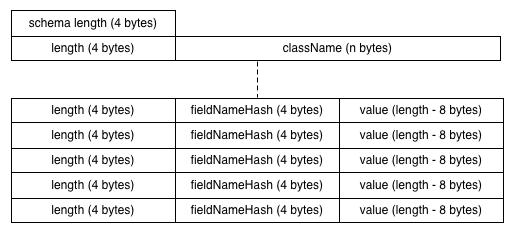
\includegraphics[width=0.75\textwidth]{schema-reference}
	\caption{The general form of serialized RemoteObjects}
	\label{fig:schema-representation}
\end{figure}

% subsection the_serialization_process (end)

\subsection{Remote Compute Service} % (fold)
\label{sub:remote_compute_service}

The remote compute service (RCS) is a simple socket server and key value store, that runs on the cloud compute platform. It's primary task is to listen for incoming invocation requests, upon receipt of a request it deserializes the target object and the argument array. These deserialized objects are synchronized with the local cache of remoted objects---Objects are sent as deltas only to prevent retransmission of information. Once the cache is synchronized the method is invoked against the target object with the argument array, and the result is in turn serialized and transmitted to the mobile device.

Deserialization is relatively straightforward, however it requires the RCS to have access to all of the class files that represent the objects that have been transmitted. This is done by simply jarring all pertinent files and having them present in the /jars folder which is located at the root of the classpath of the RCS. A single object is deserialized by loading it's class by name, and reflectively instantiating it. This requires that all RemoteObject have a null constructor (an constructor with no arguments). After which fields are looked up by the hash value of their field name and set to the serialized value.

% subsection remote_compute_service (end)

% section a_framework_for_data_migration (end)

\section{Programmer Responsibilities} 
% (fold)

% section programmer_responsibilities (end)

\section{The Model} 

% (fold)
\label{sec:the_model}

% section the_model (end)
\section{Exercising the Framework} 


\subsection{Basic Experiment} % (fold)
\label{sub:basic_experiment}

The first and most simple experiment will be used to determine if it is possible to obtain more than marginal gains in terms of battery life and computation time (over all number of computations executed in the given battery life) using a non heuristically or stochastically based model, but rather by simply shipping the computation off to a server with greater capabilities. 

% subsection basic_experiment (end)

% (fold)
\label{sec:exercising_the_framework}

% section exercising_the_framework (end)
% chapter design_modelling (end)
\chapter{Experimental Results} 

% (fold)
\label{chap:experimental_results}

% chapter experimental_results (end)
\chapter{Conclusion} 

% (fold)
\label{chap:conclusion}

\section{Summary of Contribution} 

% (fold)
\label{sec:summary_of_contribution}

% section summary_of_contribution (end)
\section{Future Work} 

% (fold)
\label{sec:future_work}

% section future_work (end)
% chapter conclusion (end)
%% This changes the headings and chapter titles (no numbers for
%% example).
\backmatter

%% This file is setup to use a bibtex file sample.bib and uses the
%% plain style.  Other styles may be used depending on the conventions
%% of your field of study.
%%
%%% Note: the bibliography must come before the appendices.
\bibliographystyle{plain} 
\bibliography{sample}

%% Use this to reset the appendix counter.  Note that the FoGS
%% requires that the word ``Appendices'' appear in the table of
%% contents either before each appendix lable or as a division
%% denoting the start of the appendices.  We take the latter option
%% here.  This is ensured by making the \texttt{appendicestoc} option
%% a default option to the UBC thesis class.
%%% If you only have one appendix, please uncomment the following line.
% \renewcommand{\appendicesname}{Appendix}
\appendix 
\chapter{First Appendix}
\begin{table}
	\begin{tabular*}{0.75\textwidth}{| c | c | c | } 
		\hline 
			Type & Data Size & Effect On Schema \\
		\hline
			byte or Byte & 1 & 5 \\
		\hline
			char or Character & 2 & 6 \\
		\hline
			short or Short & 2 & 6 \\
		\hline
			float, Float, int, or Integer & 4 & 8 \\
		\hline
			double, Double, long, or Long & 8 & 12 \\
		\hline
			byte[length] & 1 * length & 1 * length + 4 \\
		\hline
			char[length] & 2 * length & 2 * length + 4 \\
		\hline
			float[length] or int[length] & 4 * length & 4 * length + 4 \\
		\hline
			double[length] or long[length] & 8 * length & 8* length + 4 \\
		\hline
			object (not visited) & object.size() & object.size() + 8 \\
		\hline
			object (visited) & object.size() & 8 \\
		\hline
	\end{tabular*}
	\caption{Table of field sizes} 
	\label{tab:field_sizes} 
\end{table}

\chapter{Second Appendix} Here is the second appendix.

\end{document} 
\endinput

%%
%% End of file `ubcsample.tex'.
